\documentclass{article}
\usepackage{graphicx} % Required for inserting 
\usepackage{amsmath,amsfonts,amssymb}
\usepackage{float}
\usepackage{tikz}
\usetikzlibrary{automata, positioning, arrows.meta, fit, shapes.geometric}
\usepackage{amsthm}
\usepackage[colorlinks=true, allcolors=blue]{hyperref}
\newtheorem{theorem}{Theorem}[section]
\newtheorem{lemma}[theorem]{Lemma}
\theoremstyle{definition} 
\setlength{\parindent}{0pt}
\setlength{\parskip}{1em}
\newtheorem{defn}{Definition}[section]
\title{Minimal DFA's for Divisibility Testing (LSB first)}
\author{Jez Snelson \& Joshua Obayomi}
\begin{document}
\maketitle
\section{Introduction}
% Talk about
\section{Non-Distinguishability Criteria}
% Declare function r_b(x) at some point
% Declare distinguishability equivalence relation for divisibility by p ~_{d,p}
In order to write this proof we have to define a way of working with binary strings $s_x\in\{0,1\}$ such that we can assign a value to them based on the Least Significant Bit first processing order.\\
\begin{defn} 
  We define the value of a binary string according to LSB first as\\
  \[val(s_x)=val(c_1\circ c_2\circ\dots\circ c_n)=2^0\times c_1+2^1\times c_2+\dots+2^{n-1}\times c_n\ c_1,c_2,\dots,c_n\in\{0,1\}\]
\end{defn}
We want to determine the minimal amount of states for Divisibility Testing a binary string by a number $p$. To start with we want to declare our alphabet $\{0,1\}$, in this paper we will denote binary strings as $s_x\in\{0,1\}^*$ and their corresponding values $x\in\mathbb N$ (also notated as $val(s_x)$). For our accepting criteria we have that $s_x$ is accepting if $val(s_x)=x\equiv 0\ \text{(mod } p)$\\ 
In order to prove we have a minimal amount of states we rely on the Myhill Nerode Theorem and so the first thing we must do is reason with non distinguishability criteria.\\
\begin{defn} 
  We say that two strings $s_x,s_y$ are non distinguishable if and only if $\forall s_w \in \Sigma^*$ the run of $s_x\circ s_w$ is accepting if and only if the run of $s_y \circ s_w$ is accepting.\\
\end{defn}
And so with respect to our problem we have that two binary strings $s_x,s_y$ are non distinguishable if and only if  $\forall s_w \in \{0,1\}^*$ $val(s_x\circ s_w)\equiv 0 \iff val(s_y\circ s_w)\equiv 0$
\subsection{Initial ND Criteria}
\begin{defn}
  We define the residue of a string with respect to a certain base $b$ to be\\
  \[r_b(s_x)=2^{|x|}\]
\end{defn}
\begin{lemma}
  \label{2.1}
  % Define notation of x = val(s_x)
  The binary strings $s_x,s_y$ are non distinguishable if and only if\\
  $\forall w\in\mathbb N$ $r_2(s_x)w+x\equiv0\iff r_2(s_y)w+y\equiv0$
\end{lemma}
\begin{proof}
  We can work with the definition of the value function, if we have that $s_x=c_{s_x,1}\circ c_{s_x,2}\circ\dots\circ c_{s_x,|s_x|}$ $s_y=c_{s_y,1}\circ c_{s_y,2}\circ\dots\circ c_{s_y,|s_y|}$ then if we pick $s_w=c_{s_w,1}\circ c_{s_w,2}\circ\dots\circ c_{s_w,|s_w|}$ we get that if and only if they are non distinguishable then\\
  \[val(s_x\circ s_w)\equiv 0 \iff val(s_x\circ s_w)\equiv 0\text{   (mod }p)\]
  \[val(c_{s_x,1}\circ\dots\circ c_{s_x,|s_x|}\circ c_{s_w,1}\circ\dots\circ c_{s_w,|s_w|})\equiv 0\text{   (mod }p)\]\[ \iff val(c_{s_y,1}\circ \dots\circ c_{s_y,|s_y|}\circ c_{s_w,1}\dots\circ c_{s_w,|s_w|})\equiv 0\text{   (mod }p)\]
  \[c_{s_x,1}+\dots+ 2^{|s_x|-1}c_{s_x,|s_x|}+ 2^{|s_x|}c_{s_w,1}+\dots+ 2^{|s_x|+|s_w|-1}c_{s_w,|s_w|}\equiv 0 \text{   (mod }p)\]\[\iff c_{s_y,1}+\dots+ 2^{|s_y|-1}c_{s_y,|s_y|}+ 2^{|s_y|}c_{s_w,1}+\dots+ 2^{|s_y|+|s_w|-1}c_{s_w,|s_w|}\equiv 0\text{   (mod }p)\]
  We can then factor our $r_2(s_x)$ from the characters of $s_w$ to get\\
  \[r_2(s_x)val(s_w)+val(s_x)\equiv0\iff r_2(s_y)val(s_w)+val(s_y)\equiv0\text{   (mod }p)\]
  And finally replacing the values of single binary strings with their letters we get $w=val(s_w)\in\mathbb N$\\
  \[r_2(s_x)w+x\equiv0\iff r_2(s_y)w+y\equiv0\text{   (mod }p)\]
\end{proof}
\subsection{Revised ND Criteria}
\begin{lemma}
  \label{2.2}
  For all $\alpha\in\mathbb Z/p\mathbb Z$ there exists $\alpha^{-1}\in \mathbb Z/p\mathbb Z$ such that\\ $a\times a^{-1} \equiv 1\ \text{(mod p)}$ if $a,p$ are coprime and $a\neq0$
\end{lemma}
\begin{proof}
If we pick $a$ and we have that $\alpha$ and $p$ are coprime we have by Bezout's identity we have that there exists integers $x$ and $y$ such that $\alpha x+py=1$ which implies that\\ 
\[\alpha x+py\equiv\alpha x+0\equiv\alpha x\equiv1\text{   (mod }p)\]\\
And so we take $\alpha^{-1}=x$ which fulfills our required properties
\end{proof}
\begin{lemma}
  \label{2.3}
 The strings $s_x,s_y$ are non distinguishable if and only if\\
 $(r_2(s_x))^{-1}x\equiv (r_2(s_y))^{-1}y \text{  (mod p)}$
 Where $p$ is odd
\end{lemma}
\begin{proof}
  If we pick $w\in\mathbb N$ we have from \ref{2.1} that the strings $s_x, s_y$ are distinguishable if and only if\\
  \[r_2(s_x)w+x\equiv0\iff r_2(s_y)w+y\equiv0\text{   (mod }p)\]
  On both sides of the $\iff$ since $p$ is odd we have that $r_2(s_x)$ and $r_2(s_y)$ have inverses under $\text{(mod }p)$ and so we can divide through by them\\
  \[w+(r_2(s_x))^{-1}x\equiv0\iff w+(r_2(s_y))^{-1}y\equiv0\text{   (mod }p)\]
  \[(r_2(s_x))^{-1}x\equiv-w\iff (r_2(s_y))^{-1}y\equiv-w\text{   (mod }p)\]
  \[(r_2(s_x))^{-1}x\equiv (r_2(s_y))^{-1}y \text{   (mod }p)\]
\end{proof}
\section{Equivalence Relation Classes}
As we have shown our distinguishability equivalence relation $_{d,p}$ is equivalent to $r_2(s_y)x\equiv r_2(s_x)y \text{  (mod }p)$ and we want to construct our distinguishing set from this which leads us to.\\
\begin{lemma}
  The amount of equivalence classes under the non distinguishability equivalence relation $=_{d,p}$ is exactly $p$\\
  Also said as $\Sigma^*/ND=p$
\end{lemma}
\begin{proof}
  Firstly since there is only $p$ possible values for the numbers to be congruent to mod $p$ as they are integers we have that the amount of equivalence classes is $\leq p$.\\
  Now all we need to do is find $p$ possible equivalence classes of distinguishability which will force it to be $p$.\\
  Consider the strings of $0$ to $p-1$.\\
  Prepend 0s to the start of these strings to make them all the same length so we have $r_2(s_x)=\alpha$ for all of them.\\
  We then have that they are all distinct under $=_{d,p}$ as for any two such strings $s_x,s_y,x\neq y$  assuming they are non distinguishable we have by \ref{2.3} \\
  \[(r_2(s_x))^{-1}x\equiv (r_2(s_y))^{-1}y \text{  (mod p)}\]
  \[\alpha^{-1}x\equiv \alpha^{-1}y \text{  (mod p)}\]
  \[x\equiv y \text{  (mod p)}\]
  This forms a contradiction as we picked them to be distinct numbers between $0$ and $p-1$ and so they must all be distinguishable and hence in different equivalence classes.\\
  Thus we have found $p$ distinct equivalence classes and so the amount of equivalence classes is exactly $p$.
\end{proof}

\section{Even Numbers}
Now we aim to extend our Minimal DFA's to work with even numbers specifically numbers of the form $2^\alpha p$ where $\alpha,p\in\mathbb N$ and p is odd.\\
\subsection{Construction}
We will construct a proposed minimal DFA and prove that it works aswell as proving minimality.\\
\subsubsection{Checking for Divisibility by 2$^\alpha$}
Firstly it is easy to see that for checking if a binary string is divisible by $2^\alpha$ you only need to check the first $\alpha$ digits and so we can construct a DFA for that fairly easily.\\
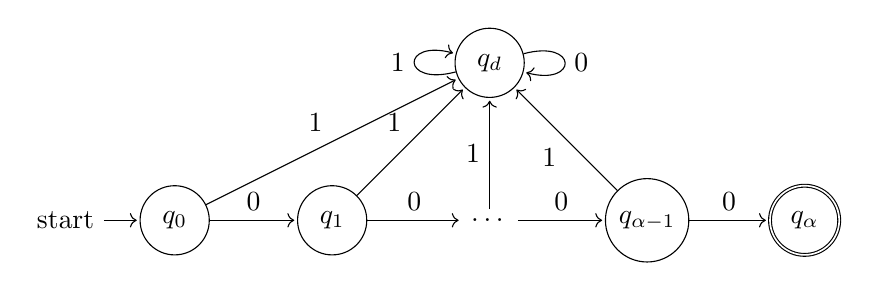
\begin{tikzpicture}[shorten >=1pt, node distance=2cm, on grid, auto]
   % First two states
   \node[state, initial] (q0) {$q_0$};
   \node[state] (q1) [right=of q0] {$q_1$};
   
   % The Dots (Ellipsis)
   \node (dots) [right=of q1] {$\dots$};
   
   % Last two states
   \node[state] (qn-1) [right=of dots] {$q_{\alpha-1}$};
   \node[state, accepting] (qn) [right=of qn-1] {$q_\alpha$};

   \node[state] (qd) [above=of dots] {$q_d$};

   % Transitions
   \path[->] 
    (q0) edge node {0} (q1)
    (q1) edge node {0} (dots)
    (dots) edge node {0} (qn-1)
    (qn-1) edge node {0} (qn)
    (q0) edge node {1} (qd)
    (q1) edge node {1} (qd)
    (dots) edge node {1} (qd)
    (qn-1) edge node {1} (qd)
    (qd) edge[loop left] node {1} (qd)
    (qd) edge[loop right] node {0} (qd);
\end{tikzpicture}
\\
Next we can construct a DFA as a joining of those two DFAs because if the first $\alpha$ digits are 0s that doesnt affect the divisibility by $p$.\\\\
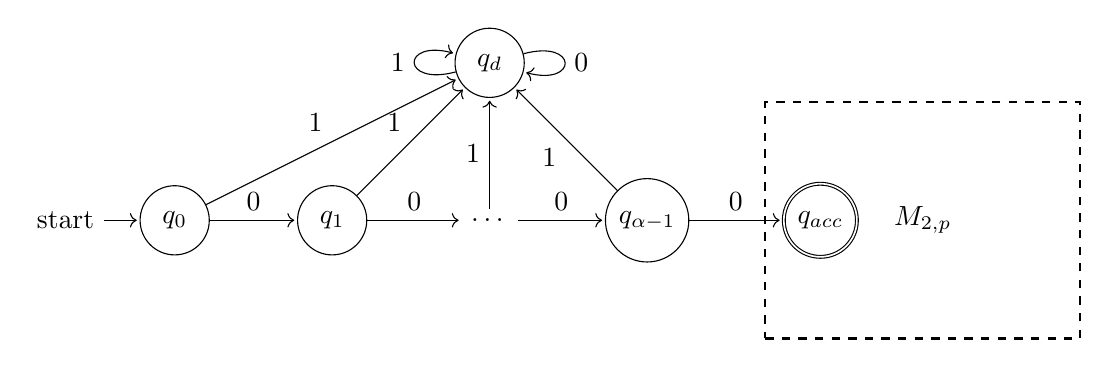
\begin{tikzpicture}[shorten >=1pt, node distance=2cm, on grid, auto]
   % First two states
   \node[state, initial] (q0) {$q_0$};
   \node[state] (q1) [right=of q0] {$q_1$};
   
   % The Dots (Ellipsis)
   \node (dots) [right=of q1] {$\dots$};
   
   % Last two states
   \node[state] (qn-1) [right=of dots] {$q_{\alpha-1}$};

   \node[state, accepting] (q_acc) [right=2.2cm of qn-1] {$q_{acc}$};
   \node[draw, dashed, minimum width=4cm, minimum height=3cm, thick] (dfa2) [right=3.5cm of qn-1] {$M_{2,p}$};

   \node[state] (qd) [above=of dots] {$q_d$};

   % Transitions
   \path[->] 
    (q0) edge node {0} (q1)
    (q1) edge node {0} (dots)
    (dots) edge node {0} (qn-1)
    (qn-1) edge node {0} (q_acc)
    (q0) edge node {1} (qd)
    (q1) edge node {1} (qd)
    (dots) edge node {1} (qd)
    (qn-1) edge node {1} (qd)
    (qd) edge[loop left] node {1} (qd)
    (qd) edge[loop right] node {0} (qd);
\end{tikzpicture}
\subsection{Proof of it working}
\begin{lemma}
  For any binary string $s_w$ the run of $s_w$ on $M_{2,2^\alpha p}$ is accepting if and only if $s_w$ is divisible by $2^\alpha p$
\end{lemma}
\begin{proof}
  We know from our previous work that $M_{2,p}$ accepts a string $s_d$ if and only if the string is divisible by $p$.\\
  All strings that are divisible by $2^\alpha p$ have the value of $2^\alpha d$ for any $s_d$ divisible by $p$ and because of this we can write any string divisible by $2^\alpha p$ as $s_w=0^\alpha \circ s_d$ for some $s_d$ divisible by $p$. If we partially calculate where the run on $M_{2,2^\alpha p}$ will end up at after processing $0^\alpha$ we get that it ends up at the start state (also the accepting state) of $M_{2,p}$ and then since $s_d$ is divisible by $p$ the run from the start state of $M_{2,p}$ will be accepting and so we have proven the machine for all $s_w$\\ 
\end{proof}
\subsection{Reachability}
% 2^\alpha to get to the start then the pick a number from the equivalence class to get to the state
\begin{lemma}
  For all $q_m$ in the states of $M_2,2^\alpha p$ there exists a string $s_w$ such that the run of $s_w$ ends at $q_m$ 
\end{lemma}
\begin{proof}
  We split $q_m$ into cases based on which part of the DFA it is in, we consider 3 cases.\\
  Case 1: $q_m$ is in the $2^\alpha$ part of the DFA $0\leq m \leq \alpha-1$ then the string is just $s_w=0^m$ and we know the run of this ends at $q_m$ by definition of the $2^{\alpha}$ part of the DFA.\\
  Case 2: $q_m=q_d$ in which case the string is $s_w=1$ and we can see the run of this ends at $q_d$\\
  Case 3: $q_m$ is a state in $M_{2,p}$ in which case we can construct $s_w$ by first taking the string $0^\alpha$ which will take us to the accepting state (also the start state of $M_{2,p}$) and then concatenating it with a string from the equivalence class of $q_m$ and so we can the run of this ends at $q_m$ by definition of $M_{2,p}$
\end{proof}
\subsection{Distinguishability}
% Odd = in p machine
% Even = in 2^\alpha machine
% Prove any odd state has a string that makes it acceptable
% Odd/Even vs Dead by string that accepts them
% Even - Odd by 1 then string that accepts the state odd gets to
% Even - Even by smallest accepting string 
\begin{lemma}
  \label{4.3}
  For all $q_m$ in the states of $M_{2,2^\alpha p}$ where $q_m\neq q_d$ we have that there exists a string $s_w$ such that running the string $w$ from $q_m$ we get to the accepting state.\\
\end{lemma}
\begin{proof}
  We split $q_m$ into cases based on which part of the DFA it is in, we consider 2 cases.\\
  Case 1: $q_m$ is in the $2^\alpha$ part of the dfa $0\leq m\leq\alpha-1$, if this is the case we have the trivial string of $s_w=0^{\alpha-m}$ which we can see will go to the accepting state.\\
  Case 2: $q_m$ is a state in $M_{2,p}$ if this is the case we know that after running the string $s_w$ at the state the value will be $r_2(s_x)w+x$ and so all we need to do is find a string $s_w$ such that $w\equiv-(r_2(s_x))^{-1}x$ which we know we can find as $r_2(s_x)^{-1}$ must exist by \ref{2.2}
\end{proof}
\begin{lemma}
  For all $q_m$ $q_n$ in the states of $M_{2,2^\alpha p}$ $m\neq n$ we have that $q_m$ is distinguishable from $Sqn$
\end{lemma}
\begin{proof}
  We split $q_m$ and $q_n$ into cases based on which part of the DFA they are in we consider 3 cases for each of them being the dead state $q_d$, being any other state in the divisibility by $2^\alpha$ part $q_l, 0\leq l\leq\alpha-1$ or being any state in $M_{2,p}$.\\
  Case 1: $q_m\neq q_d$ and $q_n=q_d$. In this case we have that the distinguishing string is the accepting string of $q_m$ which we know exists from \ref{4.3} with this $q_m$ will go to the accepting state and $q_n$ will stay at the dead state and so they are distinguishable.\\
  Case 2: $q_m$ is in the $2^\alpha$ part of the dfa $0\leq m\leq\alpha-1$ and $q_n$ in the states of $M_{2,p}$, in this case for our distinguishing string we first take 1 which will take $q_m$ to $q_d$ and $q_n$ to another state in $M_{2,p}$ as no transitions leave the machine. We then take the rest of the distinguishing string to be the accepting string of the state $q_n$ goes to and then we have that the run on $q_n$ will be accepting and the run on $q_m$ will go to the dead state and stay there and so they are distinguishable.\\
  Case 3: $q_m,q_n$ are both in the $2^\alpha$ part of the dfa $0\leq m,n\leq\alpha-1$, in this case the distinguishing string is $0^{\alpha-\max{m,n}}$ which will take the state the closest to the accepting state to the accepting state and leave the other state still in the $2^\alpha$ part of the DFA and so these states are distinguishable.\\
  Case 4: $q_m,q_n$ are both in $M_{2,p}$ we know these states are all distinguishable from our construction of the machine using equivalence clases.\\
\end{proof}
Finally since we have that our proposed machine $M_{2,2^\alpha p}$ works for testing divisibility and all states are reachable and pairwise distinguishable we have that it must be minimal and that the minimum amount of states for checking LSB first divisibility of a binary string by a number in the form $2^\alpha p$ is $p + \alpha + 1$

\end{document}